% \begin{abstract}
%   Advances in computational cognitive neuroimaging research are
%   related to the availability of large amounts of labeled brain
%   imaging data, but such data are scarce and expensive to generate.
%   While powerful data generation mechanisms, such as Generative Adversarial Networks (GANs),  have been designed  in the last decade for computer vision, such improvements have not yet carried over to brain imaging.
%   %
%   A likely reason is that GANs training is ill-suited to the noisy, high-dimensional and small-sample data available in functional neuroimaging.
%   %
%   In this paper, we introduce Conditional Independent Components Analysis (Conditional ICA): a fast functional Magnetic Resonance Imaging (fMRI) data augmentation technique, that leverages abundant resting-state data to create condica by sampling from an ICA decomposition. We then propose a mechanism to condition the generator on classes observed with few samples.
%   We first show that the generative mechanism is successful at
%   synthesizing data indistinguishable from observations, and that it yields   gains in classification accuracy in brain decoding problems. In particular
%   it outperforms GANs while being much easier to optimize and interpret. Lastly, Conditional ICA enhances classification accuracy in eight
%   datasets without further parameter tuning.



% \end{abstract}

\section{Introduction}

As a non-invasive brain imaging technique, task fMRI records brain
activity while participants are
performing specific cognitive tasks.

Univariate statistical methods, such as general linear models (GLMs)
\cite{friston1995analysis} have been successfully applied to
identifying the brain regions involved in specific tasks.
%
However such methods do not capture well correlations and interactions between brain-wide measurements.

By contrast, classifiers trained 
to \emph{decode} brain maps, i.e to discriminate between specific stimulus or task types~\cite{shirer_decoding_2012,varoquaux_how_2014,loula_decoding_2018}, take these correlations into account. 
%
The same framework is also popular for individual imaging-based diagnosis.

%
However, the large sample-complexity of these classifiers currently limits their accuracy.
%

To tackle this problem, data generation is an attractive approach, as
it could potentially compensate for the shortage of data.
Generative Adversarial Networks (GANs) are promising generative
models~\cite{goodfellow2014generative}.
% 
However, GANs are ill-suited to the noisy, high-dimensional and
small-sample data available in functional neuroimaging. 
%
Furthermore the training of GANs is notoriously unstable and there are many hyper-parameters to tune.
%


In this work, we introduce Conditional ICA: a novel data augmentation technique using ICA together with conditioning mechanisms to generate surrogate brain imaging data and improve image classification performance.
%
Conditional ICA starts from a generative model of resting state data (unconditional model), that is fine-tuned into a conditional model that can generate task data. 
%
This way, the generative model for task data benefits from the abundant
resting state data and can be trained with few labeled samples.
%
We first show that the generative model of resting state data shipped in Conditional
ICA produces samples that neither linear nor non-linear classifiers are able to distinguish.
%
Then we benchmark Conditional ICA as a generative model of task data against
various augmentation methods including GANs and conditional GANs~\cite{mirza2014conditional} on their
ability to improve classification accuracy on a large task fMRI dataset. We find that Conditional ICA yields highest accuracy improvements.
Lastly, we show on 8 different datasets that the use of Conditional ICA results in systematic improvements in classification accuracy ranging from 1\% to 5\%.


\begin{figure}
\centerline{\includegraphics[width=1\textwidth]{condica/conceptual_figure_1_v6_redim.pdf}}
\caption{\textbf{Conditional ICA approach.} Our method aims to
  generate surrogate data from Task and Rest fMRI data by synthesizing
  statistical maps that qualitatively fit the distribution of the
  original maps. These can be used to improve the accuracy of
  machine learning models that identify contrasts from the
  corresponding brain activity patterns.}
\label{Fig0}
\end{figure}



\section{Methods}

\paragraph{Notations}
We write matrices as bold capital letters, vectors as bold small letters.
$X^{\dagger}$ refers to the Moore-Penrose pseudo inverse of matrix $X$,
, $\tr(X)$ refers to the trace of matrix $X$ and
$I_k$ refers to the identity matrix in $\mathbb{R}^{k, k}$. $\mathbf{0}_k$ refers to
the null vector in $\mathbb{R}^k$.

\paragraph{Spatial Dimension reduction.} 
The outline of the proposed approach is presented in Fig.\ref{Fig0}.
%
While brain maps are high-dimensional, they span a smaller space than that of
the voxel grid. 
%
For the sake of tractability, we reduce the dimension of the data by projecting the voxel values on the
high-resolution version of the Dictionaries of Functional Modes \emph{DiFuMo}
atlas \cite{dadi_fine-grain_2020}, i.e. with $p=1024$ components.
%
The choice of dimension reduction technique generally has an impact on the
results. However we consider this question to be out of the scope of the current study and leave this to future work.

\paragraph{Unconditional generative model (resting state data generation)}
Given a large-scale resting-state dataset $X^{rest}$ in $\mathbb{R}^{p,n}$ where $n$ is the number of condica (samples) and $p=1024$ the number of components in the atlas, let us consider how to learn its distribution.
%
Assuming a Gaussian distribution is standard in this setting, yet, as
shown later, it misses key distributional features.
%
Moreover, we consider a model that subsumes the distribution of any type of
fMRI data (task or rest): a linear mixture of $k \leq p$ independent temporal signals.
%
We therefore use temporal ICA to learn a dimension reduction and unmixing matrix
$W^{rest} \in \mathbb{R}^{k, p}$ such that the $k$ sources i.e the $k$ components of
$S^{rest} = W^{rest} X^{rest}$ are as
independent as possible.
%
 
%

A straightforward method to generate new rest data would be to
independently sample them from the distribution of the sources.
%
This is easy because such distribution has supposedly independent marginals.
We apply an invertible quantile transform $q^{rest}$ to the sources $S^{rest}$ so that
the distribution of $\zb^{rest} =
q^{rest}(\sbb^{rest})$ has standardized Gaussian marginals. Since the distribution of
$\zb^{rest}$ has independent marginals, it is given by $\mathcal{N}(\zero_k, I_k)$
from which we can easily sample.
As shown later, this approach fails: such samples are still separable
from actual rest data.
%

We hypothesize that this is because independence does not hold, and
thus a latent structure among the marginals of the source distribution has to be taken into account. Therefore we assume that the distribution of $\zb^{rest}$ is given
by $\mathcal{N}(\zero_k, \Lambda^{rest})$ where $\Lambda^{rest}$ is a definite positive matrix.

$\Lambda^{rest}$ can easily be learned from a standard shrunk covariance
estimator: $\Lambda^{rest} = SSigma^{rest} (1 - \alpha) + \alpha \tr(SSigma^{rest}) I_k$ where
$\alpha$ is given by the Ledoit-Wolf formula \cite{ledoit2004well} and
$SSigma^{rest}$ is the empirical covariance of $Z^{rest}$.

Our encoding model for rest data is therefore given by \\ 
$Z^{rest} =
q^{rest}(W^{rest} X^{rest})$ and we assume that the the
distribution of $Z^{rest}$ is $\mathcal{N}(\zero_k, \Lambda_k)$.
The generative model is given by the pseudo inverse of the encoding model:
$\tilde{X}^{rest} = (W^{rest})^{\dagger} (q^{rest})^{-1}(\eps)$ where $\eps \sim
\mathcal{N}(\zero_k, \Lambda^{rest})$. 


\paragraph{Conditional generative model (generative model for task data)}
While resting state datasets have a large number of samples ($10^4 \sim 10^5$), task datasets   have a small number of samples ($10 \sim 10^2$). As a result, there are too few samples to learn high quality unmixing matrices. 
%
Therefore, using  the unmixing matrix $W^{rest}$ learned from the resting state data, we rely on the following nonlinear generative model for brain maps in a certain class $c$:
\begin{equation}
  \xb_c = (W^{rest})^{\dagger} q^{-1}(\eps)
\end{equation}
with $\eps \sim \mathcal{N}(\mub_c, \Lambda)$.

In order to maximize the number of samples used to learn the parameters of the
model, we assume that the quantile transform $q$ and the latent covariance
$\Lambda$ do not depend on the class $c$. However, the mean $\mub_c$, that can be learned efficiently using just a few tens of samples, depends on class $c$.

An overview of our generative method is shown in Fig.~\ref{Fig11}.
%
\begin{figure}
\centerline{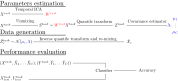
\includegraphics[width=1\textwidth]{figures/condica/method_figure}}
\caption{\textbf{Conditional ICA approach in depth.} 
The approach proceeds by learning a temporal ICA of rest data $X^{rest} \in
\mathbb{R}^{p, n}$ , resulting in
independent sources and unmixing matrix $W^{rest} \in \mathbb{R}^{k, p}$.
%
Applying the unmixing matrix to the task data, we obtain samples in the source
space $S^{task} \in \mathbb{R}^{k, n}$.
%
Afterwards, we map $S^{task}$ to a normal distribution, yielding $Z^{task} \in
\mathbb{R}^{k, n}$. 
%
Then, we estimate the covariance $\Lambda \in \mathbb{R}^{k, k}$ (all classes are assumed to have the
same covariance) and the class-specific means $\boldsymbol{\mu}_1, \dots, \mub_C \in \mathbb{R}^{k}$ according to Ledoit-Wolf's method.
%
For each class $c$, we can draw random samples $\tilde{Z}^{task}_c \in
\mathbb{R}^{k, n_{\mathrm{fakes}}}$ from the
resulting multivariate Gaussian distribution $\mathcal{N}(\mub_c, \Lambda)$ and
obtain fake data $\tilde{X}_c  \in
\mathbb{R}^{p, n_{\mathrm{fakes}}}$
by applying the inverse quantile transform and re-mixing the data using the pseudo inverse of the unmixing matrix.
%
We append these synthetic data to the actual data to create our new augmented
dataset on which we train classifiers.}
\label{Fig11}
\end{figure}
%

\section{Related work}
In image processing, data augmentation is part of standard toolboxes and
typically includes operations like cropping, rotation, translation.
%
On fMRI data these methods do not make much sense as brain condica are not invariant to such transformations.
%
More advanced techniques~\cite{zhuang2019fmri}%\cite{sandfort2019data}
are based on generative models such as GANs or variatonal
auto-encoders~\cite{kingma2013auto}. Although GAN-based method are powerful they are slow and difficult to train~\cite{arjovsky_wasserstein_2017}. In
appendix Table~\ref{app:runningtime:tab}, we show that Conditional ICA is several orders of magnitude faster than GAN-based methods.

Our method is not an adversarial procedure, however it relates to other
powerful generative models such as variatonal
auto-encoders~\cite{kingma2013auto} with which it shares strong similarities.
Indeed the analog of the encoding function in the variational auto-encoder is
given by $e(\xb) = \Lambda^{-\frac12}q(W^{rest} \xb)$ in our model and the analog to the decoding
function in the variational auto-encoder is given by $d(\zb) =
(W^{rest})^{\dagger}q^{-1}(\Lambda^{\frac12}\zb)$ in our model. As in the variational auto-encoder, $e$ approximately maps the distribution of the data to a standardized Gaussian distribution,
while the reconstruction error defined by the difference in l2 norm
$\|d(e(\xb)) - \xb\|^2_2$ must remain small.
Lastly, another classical generative model related to ours is normalizing
flows.  We note that when $W^{rest}$ is squared (no dimension reduction in ICA), the decoding operator $d$ is invertible (its inverse is $e$) making our
model an instance of normalizing flows. 
%
A great property is thus the simplicity and reduced cost of data generation.


